% !TeX root = main.tex

\hypertarget{area-between-curves}{%
\section{Area Between Curves}\label{area-between-curves}}

The idea of finding area under an curve can be generalized to finding
areas between curves. That is to slice the region enclosed by the
curves, represent the area of a slice using the functions and a
differential, and then take the sum which can be expressed as an
integral.

\begin{fullwidth}
  \centering
  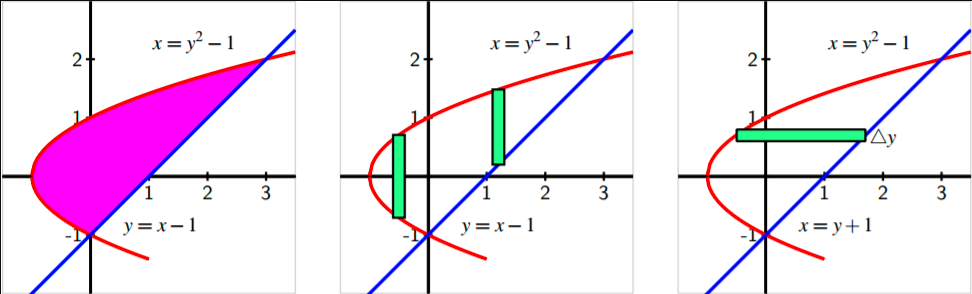
\includegraphics[width=0.8\linewidth]{img/image-20200506101055076.png}
\end{fullwidth}

\hypertarget{summarize-the-idea-we-get-the-following-strategy}{%
\subsection{Summarize the idea, we get the following
strategy}\label{summarize-the-idea-we-get-the-following-strategy}}

\begin{enumerate}[sepno]
\item
  Sketch the curves and the enclosed region.
\item
  Determine the boundaries of the region: find intersection points if
  they are on the boundary.
\item
  Draw and label the dimension of a representative slice.
\item
  State the area of the representative slice:

  \begin{itemize}
  \item
    if vertical slices are used, the area of a slice can be represented
    by \(\lvert U(x)-L(x)\rvert\, dx\), where \(U(x)\) and \(L(x)\) are
    the upper and lower curves respectively;
  \item
    if horizontal slices are used, the area of a slice can be
    represented by \(\lvert R(y)-L(y)\rvert\, dy\), where \(R(y)\) and
    \(L(y)\) are the right and left curves respectively;
  \end{itemize}
\item
  Write a definite integral to represent area:

  \begin{itemize}
  \item
    if vertical slides:
    \(\displaystyle\int^{x_R}_{x_L}\lvert U(x)-L(x)\rvert\, dx\), where
    \(x_L\) and \(x_R\) are the left and right boundaries of the region.
  \item
    if horizontal slides:
    \(\displaystyle\int^{y_U}_{y_L}\lvert R(y)-L(y)\rvert\, dy\)
  \end{itemize}
\end{enumerate}

\begin{example}

Find the area between \(f(x)= -x^2+4x\) and \(g(x)=x^2-6x+5\) over the
interval \(0\le x\le 1\).

\end{example}
\vspace*{6\baselineskip}

\begin{example}

Find the area enclosed by \(y=x-4\), \(y=-x^2 - 3x - 1\), and \(x= - 1\) .

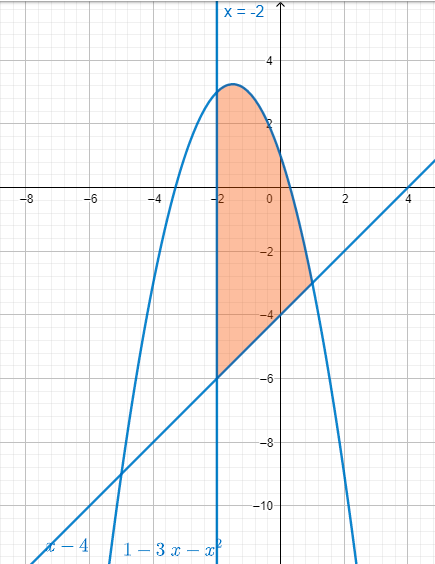
\includegraphics[scale=0.4]{img/image-20200506104639920.png}

\end{example}
\vspace*{6\baselineskip}


\begin{example}

Find the area between \(y=\sin x\cos x\) and \(y=\sin x\),
\(-\pi/2\le x\le \pi\).

\end{example}
\vspace*{6\baselineskip}

\begin{example}

Find the area between \(x=y^2-y-5\) and \(x=y+3\).

\end{example}
\vspace*{6\baselineskip}


\begin{example}

Evaluate the integral by interpreting it as the area between two curves
\[\int_0^3|\sqrt{x+5}-x|\, dx\]

\end{example}
\vspace*{6\baselineskip}


\subsection{Practice}

\begin{exercise}

Find the area between \(y=x^2+2\) and \(y=2x+5\).

\end{exercise}
\vspace*{6\baselineskip}


\begin{exercise}

Find the area enclosed by \(y=\cos\theta\), \(y=0.5\), \(x=0\), and
\(x=\pi\).

\end{exercise}
\vspace*{6\baselineskip}


\begin{exercise}

Find the area between \(y=|x|\) and \(y=x^2\).

\end{exercise}
\vspace*{6\baselineskip}

\begin{exercise}

Find the area between \(y=x\) and \(x=y^2\).

\end{exercise}
\vspace*{6\baselineskip}

\begin{exercise}

Find the area between \(x= - 3+y^2\) and \(x=y - y^2\).

\end{exercise}
\vspace*{6\baselineskip}

\begin{exercise}

Find the area between \(y=\sin x\) and \(y=\cos x\) over \([ - \pi,\pi]\).

\end{exercise}

